\documentclass[twoside]{book}

% Packages required by doxygen
\usepackage{fixltx2e}
\usepackage{calc}
\usepackage{doxygen}
\usepackage[export]{adjustbox} % also loads graphicx
\usepackage{graphicx}
\usepackage[utf8]{inputenc}
\usepackage{makeidx}
\usepackage{multicol}
\usepackage{multirow}
\PassOptionsToPackage{warn}{textcomp}
\usepackage{textcomp}
\usepackage[nointegrals]{wasysym}
\usepackage[table]{xcolor}

% NLS support packages
\usepackage[spanish]{babel}
% Font selection
\usepackage[T1]{fontenc}
\usepackage[scaled=.90]{helvet}
\usepackage{courier}
\usepackage{amssymb}
\usepackage{sectsty}
\renewcommand{\familydefault}{\sfdefault}
\allsectionsfont{%
  \fontseries{bc}\selectfont%
  \color{darkgray}%
}
\renewcommand{\DoxyLabelFont}{%
  \fontseries{bc}\selectfont%
  \color{darkgray}%
}
\newcommand{\+}{\discretionary{\mbox{\scriptsize$\hookleftarrow$}}{}{}}

% Page & text layout
\usepackage{geometry}
\geometry{%
  a4paper,%
  top=2.5cm,%
  bottom=2.5cm,%
  left=2.5cm,%
  right=2.5cm%
}
\tolerance=750
\hfuzz=15pt
\hbadness=750
\setlength{\emergencystretch}{15pt}
\setlength{\parindent}{0cm}
\setlength{\parskip}{3ex plus 2ex minus 2ex}
\makeatletter
\renewcommand{\paragraph}{%
  \@startsection{paragraph}{4}{0ex}{-1.0ex}{1.0ex}{%
    \normalfont\normalsize\bfseries\SS@parafont%
  }%
}
\renewcommand{\subparagraph}{%
  \@startsection{subparagraph}{5}{0ex}{-1.0ex}{1.0ex}{%
    \normalfont\normalsize\bfseries\SS@subparafont%
  }%
}
\makeatother

% Headers & footers
\usepackage{fancyhdr}
\pagestyle{fancyplain}
\fancyhead[LE]{\fancyplain{}{\bfseries\thepage}}
\fancyhead[CE]{\fancyplain{}{}}
\fancyhead[RE]{\fancyplain{}{\bfseries\leftmark}}
\fancyhead[LO]{\fancyplain{}{\bfseries\rightmark}}
\fancyhead[CO]{\fancyplain{}{}}
\fancyhead[RO]{\fancyplain{}{\bfseries\thepage}}
\fancyfoot[LE]{\fancyplain{}{}}
\fancyfoot[CE]{\fancyplain{}{}}
\fancyfoot[RE]{\fancyplain{}{\bfseries\scriptsize Generado por Doxygen }}
\fancyfoot[LO]{\fancyplain{}{\bfseries\scriptsize Generado por Doxygen }}
\fancyfoot[CO]{\fancyplain{}{}}
\fancyfoot[RO]{\fancyplain{}{}}
\renewcommand{\footrulewidth}{0.4pt}
\renewcommand{\chaptermark}[1]{%
  \markboth{#1}{}%
}
\renewcommand{\sectionmark}[1]{%
  \markright{\thesection\ #1}%
}

% Indices & bibliography
\usepackage{natbib}
\usepackage[titles]{tocloft}
\setcounter{tocdepth}{3}
\setcounter{secnumdepth}{5}
\makeindex

% Hyperlinks (required, but should be loaded last)
\usepackage{ifpdf}
\ifpdf
  \usepackage[pdftex,pagebackref=true]{hyperref}
\else
  \usepackage[ps2pdf,pagebackref=true]{hyperref}
\fi
\hypersetup{%
  colorlinks=true,%
  linkcolor=blue,%
  citecolor=blue,%
  unicode%
}

% Custom commands
\newcommand{\clearemptydoublepage}{%
  \newpage{\pagestyle{empty}\cleardoublepage}%
}

\usepackage{caption}
\captionsetup{labelsep=space,justification=centering,font={bf},singlelinecheck=off,skip=4pt,position=top}

%===== C O N T E N T S =====

\begin{document}

% Titlepage & ToC
\hypersetup{pageanchor=false,
             bookmarksnumbered=true,
             pdfencoding=unicode
            }
\pagenumbering{alph}
\begin{titlepage}
\vspace*{7cm}
\begin{center}%
{\Large Gestión de intervalos \\[1ex]\large 0 }\\
\vspace*{1cm}
{\large Generado por Doxygen 1.8.13}\\
\end{center}
\end{titlepage}
\clearemptydoublepage
\pagenumbering{roman}
\tableofcontents
\clearemptydoublepage
\pagenumbering{arabic}
\hypersetup{pageanchor=true}

%--- Begin generated contents ---
\chapter{Índice de clases}
\section{Lista de clases}
Lista de las clases, estructuras, uniones e interfaces con una breve descripción\+:\begin{DoxyCompactList}
\item\contentsline{section}{\hyperlink{classIntervalo}{Intervalo} }{\pageref{classIntervalo}}{}
\end{DoxyCompactList}

\chapter{Indice de archivos}
\section{Lista de archivos}
Lista de todos los archivos documentados y con descripciones breves\+:\begin{DoxyCompactList}
\item\contentsline{section}{include/\hyperlink{intervalo_8h}{intervalo.\+h} }{\pageref{intervalo_8h}}{}
\item\contentsline{section}{src/\hyperlink{intervalo_8cpp}{intervalo.\+cpp} }{\pageref{intervalo_8cpp}}{}
\item\contentsline{section}{src/\hyperlink{main_8cpp}{main.\+cpp} }{\pageref{main_8cpp}}{}
\end{DoxyCompactList}

\chapter{Documentación de las clases}
\hypertarget{classIntervalo}{}\section{Referencia de la Clase Intervalo}
\label{classIntervalo}\index{Intervalo@{Intervalo}}
\subsection*{Métodos públicos}
\begin{DoxyCompactItemize}
\item 
\hyperlink{classIntervalo_a9b5b23dda7ee26b444898457959cb03d}{Intervalo} ()
\begin{DoxyCompactList}\small\item\em comprueba que los argumentos definen un intervalo correcto cota\+Inferior $<$= cota\+Superior \end{DoxyCompactList}\item 
\hyperlink{classIntervalo_a321e56ef7e1f4a774bd64cc2609156f4}{Intervalo} (double cota\+Inferior, double cota\+Superior)
\begin{DoxyCompactList}\small\item\em Crea un \hyperlink{classIntervalo}{Intervalo} cerrado por defecto. \end{DoxyCompactList}\item 
\hyperlink{classIntervalo_af70d523399465f51862977a303656c72}{Intervalo} (double cota\+Inferior, double cota\+Superior, bool cerrado\+Inferior, bool cerrado\+Superior)
\begin{DoxyCompactList}\small\item\em Crea \hyperlink{classIntervalo}{Intervalo}. \end{DoxyCompactList}\item 
double \hyperlink{classIntervalo_aafa3f6ec78c6bd44b568e343fb22fc90}{get\+Cota\+Inf} () const
\begin{DoxyCompactList}\small\item\em Devuelve la cota inferior del intervalo. \end{DoxyCompactList}\item 
double \hyperlink{classIntervalo_a2dd767a860e4e85ec3d5a44e78884b76}{get\+Cota\+Sup} () const
\begin{DoxyCompactList}\small\item\em Devuelve la cota superior del intervalo. \end{DoxyCompactList}\item 
bool \hyperlink{classIntervalo_aac8f7b98dd0d702086ea897f5c9ad932}{dentro\+Cota\+Inf} () const
\begin{DoxyCompactList}\small\item\em Consulta si el intervalo es cerrado en su cota inferior. \end{DoxyCompactList}\item 
bool \hyperlink{classIntervalo_aed0964a68d4b727bd104f5128ee7a7ef}{dentro\+Cota\+Sup} () const
\begin{DoxyCompactList}\small\item\em Consulta si el intervalo es cerrado en su cota superior. \end{DoxyCompactList}\item 
void \hyperlink{classIntervalo_a3e7cfa7c148a4e60be7040fecf506313}{set\+Intervalo} (double cota\+Inferior, double cota\+Superior, bool cerrado\+Inferior, bool cerrado\+Superior)
\begin{DoxyCompactList}\small\item\em Define los valores del intervalo. \end{DoxyCompactList}\item 
bool \hyperlink{classIntervalo_adc77e18147f9f9f85476a0d44257bb02}{es\+Vacio} () const
\begin{DoxyCompactList}\small\item\em Consulta si el intervalo almacenado es vacío o no. \end{DoxyCompactList}\item 
bool \hyperlink{classIntervalo_a2cccd9264f1b3912c6006fe3e2a70289}{esta\+Dentro} (double n) const
\begin{DoxyCompactList}\small\item\em Consulta si un determinado valor está dentro del intervalo. \end{DoxyCompactList}\end{DoxyCompactItemize}


\subsection{Descripción detallada}


Definición en la línea 11 del archivo intervalo.\+h.



\subsection{Documentación del constructor y destructor}
\mbox{\Hypertarget{classIntervalo_a9b5b23dda7ee26b444898457959cb03d}\label{classIntervalo_a9b5b23dda7ee26b444898457959cb03d}} 
\index{Intervalo@{Intervalo}!Intervalo@{Intervalo}}
\index{Intervalo@{Intervalo}!Intervalo@{Intervalo}}
\subsubsection{\texorpdfstring{Intervalo()}{Intervalo()}\hspace{0.1cm}{\footnotesize\ttfamily [1/3]}}
{\footnotesize\ttfamily Intervalo\+::\+Intervalo (\begin{DoxyParamCaption}{ }\end{DoxyParamCaption})}



comprueba que los argumentos definen un intervalo correcto cota\+Inferior $<$= cota\+Superior 


\begin{DoxyParams}{Parámetros}
{\em cota\+Inferior} & \\
\hline
{\em cota\+Superior} & \\
\hline
\end{DoxyParams}
\begin{DoxyReturn}{Devuelve}

\end{DoxyReturn}

\begin{DoxyRetVals}{Valores devueltos}
{\em true} & si correcto \hyperlink{classIntervalo}{Intervalo} vacio por defecto\+Sup valor\+Inf = valor\+Sup \& abierto\+Inf + abierto \\
\hline
\end{DoxyRetVals}


Definición en la línea 16 del archivo intervalo.\+cpp.


\begin{DoxyCode}
16                     \{
17   cotaInf = 0;
18   cotaSup = 0;
19   cerradoInf = \textcolor{keyword}{false};
20   cerradoSup = \textcolor{keyword}{false};
21 \}
\end{DoxyCode}
\mbox{\Hypertarget{classIntervalo_a321e56ef7e1f4a774bd64cc2609156f4}\label{classIntervalo_a321e56ef7e1f4a774bd64cc2609156f4}} 
\index{Intervalo@{Intervalo}!Intervalo@{Intervalo}}
\index{Intervalo@{Intervalo}!Intervalo@{Intervalo}}
\subsubsection{\texorpdfstring{Intervalo()}{Intervalo()}\hspace{0.1cm}{\footnotesize\ttfamily [2/3]}}
{\footnotesize\ttfamily Intervalo\+::\+Intervalo (\begin{DoxyParamCaption}\item[{double}]{cota\+Inferior,  }\item[{double}]{cota\+Superior }\end{DoxyParamCaption})}



Crea un \hyperlink{classIntervalo}{Intervalo} cerrado por defecto. 


\begin{DoxyParams}{Parámetros}
{\em cota\+Inferior} & \\
\hline
{\em cota\+Superior} & cota\+Inferior $<$= cota\+Superior \\
\hline
\end{DoxyParams}


Definición en la línea 23 del archivo intervalo.\+cpp.


\begin{DoxyCode}
23                                            \{
24   assert (valido(cinf,csup, \textcolor{keyword}{true}, \textcolor{keyword}{true}));
25     cotaInf = cinf;
26     cotaSup = csup;
27     cerradoInf = \textcolor{keyword}{true};
28     cerradoSup = \textcolor{keyword}{true};
29 \}
\end{DoxyCode}
\mbox{\Hypertarget{classIntervalo_af70d523399465f51862977a303656c72}\label{classIntervalo_af70d523399465f51862977a303656c72}} 
\index{Intervalo@{Intervalo}!Intervalo@{Intervalo}}
\index{Intervalo@{Intervalo}!Intervalo@{Intervalo}}
\subsubsection{\texorpdfstring{Intervalo()}{Intervalo()}\hspace{0.1cm}{\footnotesize\ttfamily [3/3]}}
{\footnotesize\ttfamily Intervalo\+::\+Intervalo (\begin{DoxyParamCaption}\item[{double}]{cota\+Inferior,  }\item[{double}]{cota\+Superior,  }\item[{bool}]{cerrado\+Inferior,  }\item[{bool}]{cerrado\+Superior }\end{DoxyParamCaption})}



Crea \hyperlink{classIntervalo}{Intervalo}. 


\begin{DoxyParams}{Parámetros}
{\em cerrado\+Inferior} & \\
\hline
{\em cerrado\+Superior} & \\
\hline
{\em cota\+Inferior} & \\
\hline
{\em cota\+Superior} & cota\+Inferior $<$= cota\+Superior \\
\hline
\end{DoxyParams}


Definición en la línea 31 del archivo intervalo.\+cpp.


\begin{DoxyCode}
31                                                                        \{
32   assert (valido(cinf, csup, cerrinf, cerrsup));
33     cotaInf = cinf;
34     cotaSup = csup;
35     cerradoInf = cerrinf;
36     cerradoSup = cerrsup;
37 \textcolor{comment}{//     else *this = Intervalo();}
38 \}
\end{DoxyCode}


\subsection{Documentación de las funciones miembro}
\mbox{\Hypertarget{classIntervalo_aac8f7b98dd0d702086ea897f5c9ad932}\label{classIntervalo_aac8f7b98dd0d702086ea897f5c9ad932}} 
\index{Intervalo@{Intervalo}!dentro\+Cota\+Inf@{dentro\+Cota\+Inf}}
\index{dentro\+Cota\+Inf@{dentro\+Cota\+Inf}!Intervalo@{Intervalo}}
\subsubsection{\texorpdfstring{dentro\+Cota\+Inf()}{dentroCotaInf()}}
{\footnotesize\ttfamily bool Intervalo\+::dentro\+Cota\+Inf (\begin{DoxyParamCaption}{ }\end{DoxyParamCaption}) const}



Consulta si el intervalo es cerrado en su cota inferior. 

\begin{DoxyReturn}{Devuelve}

\end{DoxyReturn}

\begin{DoxyRetVals}{Valores devueltos}
{\em true} & si es cerrado \\
\hline
{\em false} & si es cerrado \\
\hline
\end{DoxyRetVals}


Definición en la línea 48 del archivo intervalo.\+cpp.


\begin{DoxyCode}
48                                    \{
49     \textcolor{keywordflow}{return} cerradoInf;
50 \}
\end{DoxyCode}
\mbox{\Hypertarget{classIntervalo_aed0964a68d4b727bd104f5128ee7a7ef}\label{classIntervalo_aed0964a68d4b727bd104f5128ee7a7ef}} 
\index{Intervalo@{Intervalo}!dentro\+Cota\+Sup@{dentro\+Cota\+Sup}}
\index{dentro\+Cota\+Sup@{dentro\+Cota\+Sup}!Intervalo@{Intervalo}}
\subsubsection{\texorpdfstring{dentro\+Cota\+Sup()}{dentroCotaSup()}}
{\footnotesize\ttfamily bool Intervalo\+::dentro\+Cota\+Sup (\begin{DoxyParamCaption}{ }\end{DoxyParamCaption}) const}



Consulta si el intervalo es cerrado en su cota superior. 

\begin{DoxyReturn}{Devuelve}

\end{DoxyReturn}

\begin{DoxyRetVals}{Valores devueltos}
{\em true} & si es cerrado \\
\hline
{\em false} & si es cerrado \\
\hline
\end{DoxyRetVals}


Definición en la línea 52 del archivo intervalo.\+cpp.


\begin{DoxyCode}
52                                    \{
53     \textcolor{keywordflow}{return} cerradoSup;
54 \}
\end{DoxyCode}
\mbox{\Hypertarget{classIntervalo_a2cccd9264f1b3912c6006fe3e2a70289}\label{classIntervalo_a2cccd9264f1b3912c6006fe3e2a70289}} 
\index{Intervalo@{Intervalo}!esta\+Dentro@{esta\+Dentro}}
\index{esta\+Dentro@{esta\+Dentro}!Intervalo@{Intervalo}}
\subsubsection{\texorpdfstring{esta\+Dentro()}{estaDentro()}}
{\footnotesize\ttfamily bool Intervalo\+::esta\+Dentro (\begin{DoxyParamCaption}\item[{double}]{n }\end{DoxyParamCaption}) const}



Consulta si un determinado valor está dentro del intervalo. 


\begin{DoxyParams}{Parámetros}
{\em n} & El valor consultado \\
\hline
\end{DoxyParams}
\begin{DoxyReturn}{Devuelve}

\end{DoxyReturn}

\begin{DoxyRetVals}{Valores devueltos}
{\em true} & si el valor {\ttfamily n} pertenece al intervalo, \\
\hline
{\em false} & en otro caso \\
\hline
\end{DoxyRetVals}


Definición en la línea 68 del archivo intervalo.\+cpp.


\begin{DoxyCode}
68                                         \{
69     \textcolor{keywordflow}{return} ((p> cotaInf && p < cotaSup) || (p == cotaInf && cerradoInf) || (p == cotaSup && cerradoSup));
70 \}
\end{DoxyCode}
\mbox{\Hypertarget{classIntervalo_adc77e18147f9f9f85476a0d44257bb02}\label{classIntervalo_adc77e18147f9f9f85476a0d44257bb02}} 
\index{Intervalo@{Intervalo}!es\+Vacio@{es\+Vacio}}
\index{es\+Vacio@{es\+Vacio}!Intervalo@{Intervalo}}
\subsubsection{\texorpdfstring{es\+Vacio()}{esVacio()}}
{\footnotesize\ttfamily bool Intervalo\+::es\+Vacio (\begin{DoxyParamCaption}{ }\end{DoxyParamCaption}) const}



Consulta si el intervalo almacenado es vacío o no. 

\begin{DoxyReturn}{Devuelve}

\end{DoxyReturn}

\begin{DoxyRetVals}{Valores devueltos}
{\em true} & si es un intervalo vacío, \\
\hline
{\em false} & en otro caso \\
\hline
\end{DoxyRetVals}


Definición en la línea 65 del archivo intervalo.\+cpp.


\begin{DoxyCode}
65                              \{
66     \textcolor{keywordflow}{return} ((cotaInf == cotaSup) && !cerradoInf);
67 \}
\end{DoxyCode}
\mbox{\Hypertarget{classIntervalo_aafa3f6ec78c6bd44b568e343fb22fc90}\label{classIntervalo_aafa3f6ec78c6bd44b568e343fb22fc90}} 
\index{Intervalo@{Intervalo}!get\+Cota\+Inf@{get\+Cota\+Inf}}
\index{get\+Cota\+Inf@{get\+Cota\+Inf}!Intervalo@{Intervalo}}
\subsubsection{\texorpdfstring{get\+Cota\+Inf()}{getCotaInf()}}
{\footnotesize\ttfamily double Intervalo\+::get\+Cota\+Inf (\begin{DoxyParamCaption}{ }\end{DoxyParamCaption}) const}



Devuelve la cota inferior del intervalo. 

\begin{DoxyReturn}{Devuelve}
El valor de la cota 
\end{DoxyReturn}


Definición en la línea 40 del archivo intervalo.\+cpp.


\begin{DoxyCode}
40                                   \{
41     \textcolor{keywordflow}{return} cotaInf ;
42 \}
\end{DoxyCode}
\mbox{\Hypertarget{classIntervalo_a2dd767a860e4e85ec3d5a44e78884b76}\label{classIntervalo_a2dd767a860e4e85ec3d5a44e78884b76}} 
\index{Intervalo@{Intervalo}!get\+Cota\+Sup@{get\+Cota\+Sup}}
\index{get\+Cota\+Sup@{get\+Cota\+Sup}!Intervalo@{Intervalo}}
\subsubsection{\texorpdfstring{get\+Cota\+Sup()}{getCotaSup()}}
{\footnotesize\ttfamily double Intervalo\+::get\+Cota\+Sup (\begin{DoxyParamCaption}{ }\end{DoxyParamCaption}) const}



Devuelve la cota superior del intervalo. 

\begin{DoxyReturn}{Devuelve}
El valor de la cota 
\end{DoxyReturn}


Definición en la línea 44 del archivo intervalo.\+cpp.


\begin{DoxyCode}
44                                   \{
45     \textcolor{keywordflow}{return} cotaSup ;
46 \}
\end{DoxyCode}
\mbox{\Hypertarget{classIntervalo_a3e7cfa7c148a4e60be7040fecf506313}\label{classIntervalo_a3e7cfa7c148a4e60be7040fecf506313}} 
\index{Intervalo@{Intervalo}!set\+Intervalo@{set\+Intervalo}}
\index{set\+Intervalo@{set\+Intervalo}!Intervalo@{Intervalo}}
\subsubsection{\texorpdfstring{set\+Intervalo()}{setIntervalo()}}
{\footnotesize\ttfamily void Intervalo\+::set\+Intervalo (\begin{DoxyParamCaption}\item[{double}]{cota\+Inferior,  }\item[{double}]{cota\+Superior,  }\item[{bool}]{cerrado\+Inferior,  }\item[{bool}]{cerrado\+Superior }\end{DoxyParamCaption})}



Define los valores del intervalo. 


\begin{DoxyParams}{Parámetros}
{\em cerrado\+Inferior} & \\
\hline
{\em cerrado\+Superior} & \\
\hline
{\em cota\+Inferior} & \\
\hline
{\em cota\+Superior} & cota\+Inferior $<$= cota\+Superior \\
\hline
\end{DoxyParams}


Definición en la línea 56 del archivo intervalo.\+cpp.


\begin{DoxyCode}
56                                                                                 \{
57   \textcolor{keywordflow}{if} (valido(cinf, csup, cerrinf, cerrsup)) \{
58     cotaInf = cinf;
59     cotaSup = csup;
60     cerradoInf = cerrinf;
61     cerradoSup = cerrsup;    
62     \}
63 \}
\end{DoxyCode}


La documentación para esta clase fue generada a partir de los siguientes ficheros\+:\begin{DoxyCompactItemize}
\item 
include/\hyperlink{intervalo_8h}{intervalo.\+h}\item 
src/\hyperlink{intervalo_8cpp}{intervalo.\+cpp}\end{DoxyCompactItemize}

\chapter{Documentación de archivos}
\hypertarget{intervalo_8h}{}\section{Referencia del Archivo include/intervalo.h}
\label{intervalo_8h}\index{include/intervalo.\+h@{include/intervalo.\+h}}
Gráfico de los archivos que directa o indirectamente incluyen a este archivo\+:
\nopagebreak
\begin{figure}[H]
\begin{center}
\leavevmode
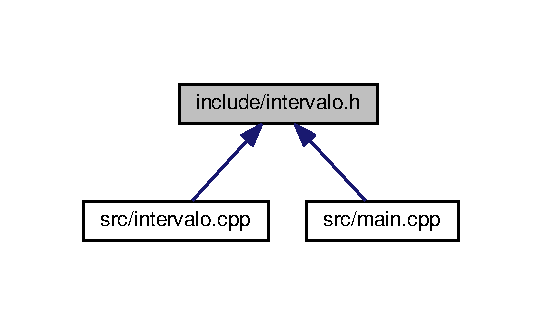
\includegraphics[width=260pt]{intervalo_8h__dep__incl}
\end{center}
\end{figure}
\subsection*{Clases}
\begin{DoxyCompactItemize}
\item 
class \hyperlink{classIntervalo}{Intervalo}
\end{DoxyCompactItemize}
\subsection*{Funciones}
\begin{DoxyCompactItemize}
\item 
\mbox{\Hypertarget{intervalo_8h_a4d876dab3159c523343e8f603af65cbb}\label{intervalo_8h_a4d876dab3159c523343e8f603af65cbb}} 
bool {\bfseries valido} (double, double, bool, bool)
\item 
\hyperlink{classIntervalo}{Intervalo} \hyperlink{intervalo_8h_ab691781bae666d71c1430e097a742ddb}{interseccion} (\hyperlink{classIntervalo}{Intervalo} i1, \hyperlink{classIntervalo}{Intervalo} i2)
\begin{DoxyCompactList}\small\item\em realiza la interseccion de dos intervalos, puede resultar un intervalo vacío en caso de que no tengan cotas comunes, en caso contrario se revisan las cotas. \end{DoxyCompactList}\item 
void \hyperlink{intervalo_8h_ae93092259c95b463d176a768b9884802}{escribir} (const \hyperlink{classIntervalo}{Intervalo} \&i)
\begin{DoxyCompactList}\small\item\em Imprime los valores de un intervalo de forma visual según lo indicado en el guión. \end{DoxyCompactList}\item 
void \hyperlink{intervalo_8h_a81ca561257a3eea794e139a64fdd6593}{leer} (\hyperlink{classIntervalo}{Intervalo} \&i)
\begin{DoxyCompactList}\small\item\em Lee los valores del intervalo según el formato indicado en el guión. \end{DoxyCompactList}\item 
void \hyperlink{intervalo_8h_a4414e0616dd83662f4b657056c06c5fe}{comprobar\+Vacio} (\hyperlink{classIntervalo}{Intervalo} i)
\begin{DoxyCompactList}\small\item\em Muestra un mensaje en pantalla indicando si el intervalo es vacío o no. \end{DoxyCompactList}\end{DoxyCompactItemize}


\subsection{Descripción detallada}
\begin{DoxyAuthor}{Autor}
decsai.\+ugr.\+es 
\end{DoxyAuthor}


\subsection{Documentación de las funciones}
\mbox{\Hypertarget{intervalo_8h_a4414e0616dd83662f4b657056c06c5fe}\label{intervalo_8h_a4414e0616dd83662f4b657056c06c5fe}} 
\index{intervalo.\+h@{intervalo.\+h}!comprobar\+Vacio@{comprobar\+Vacio}}
\index{comprobar\+Vacio@{comprobar\+Vacio}!intervalo.\+h@{intervalo.\+h}}
\subsubsection{\texorpdfstring{comprobar\+Vacio()}{comprobarVacio()}}
{\footnotesize\ttfamily void comprobar\+Vacio (\begin{DoxyParamCaption}\item[{\hyperlink{classIntervalo}{Intervalo}}]{i }\end{DoxyParamCaption})}



Muestra un mensaje en pantalla indicando si el intervalo es vacío o no. 


\begin{DoxyParams}{Parámetros}
{\em i} & El intervalo \\
\hline
\end{DoxyParams}


Definición en la línea 109 del archivo intervalo.\+cpp.


\begin{DoxyCode}
109                                   \{
110      \hyperlink{intervalo_8cpp_a4ffcdcbcf710a7461d8263cd14a32438}{escribir}(obj);
111     \textcolor{keywordflow}{if} (obj.esVacio())
112         cout << \textcolor{stringliteral}{"Vacio"};
113     \textcolor{keywordflow}{else}  cout << \textcolor{stringliteral}{"NO Vacio"};
114     cout << endl;
115 \}
\end{DoxyCode}
Gráfico de llamadas para esta función\+:
\nopagebreak
\begin{figure}[H]
\begin{center}
\leavevmode
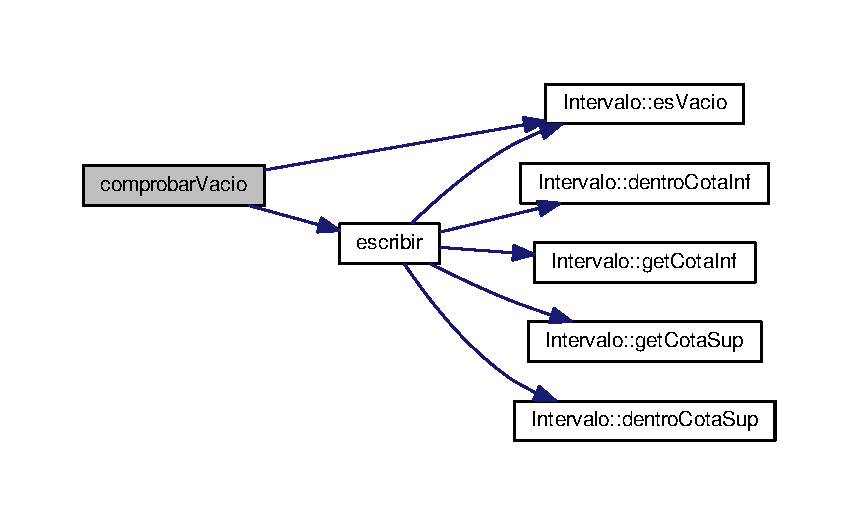
\includegraphics[width=350pt]{intervalo_8h_a4414e0616dd83662f4b657056c06c5fe_cgraph}
\end{center}
\end{figure}
\mbox{\Hypertarget{intervalo_8h_ae93092259c95b463d176a768b9884802}\label{intervalo_8h_ae93092259c95b463d176a768b9884802}} 
\index{intervalo.\+h@{intervalo.\+h}!escribir@{escribir}}
\index{escribir@{escribir}!intervalo.\+h@{intervalo.\+h}}
\subsubsection{\texorpdfstring{escribir()}{escribir()}}
{\footnotesize\ttfamily void escribir (\begin{DoxyParamCaption}\item[{const \hyperlink{classIntervalo}{Intervalo} \&}]{i }\end{DoxyParamCaption})}



Imprime los valores de un intervalo de forma visual según lo indicado en el guión. 


\begin{DoxyParams}{Parámetros}
{\em El} & intervalo \\
\hline
\end{DoxyParams}


Definición en la línea 77 del archivo intervalo.\+cpp.


\begin{DoxyCode}
77                                      \{
78     \textcolor{keywordflow}{if} (obj.esVacio())
79         cout << \textcolor{stringliteral}{"0 !!"};
80     \textcolor{keywordflow}{else} \{
81         \textcolor{keywordflow}{if} (obj.dentroCotaInf())
82          cout << \textcolor{charliteral}{'['};
83         \textcolor{keywordflow}{else} cout << \textcolor{charliteral}{'('};
84         cout << obj.getCotaInf() << \textcolor{stringliteral}{","} << obj.getCotaSup();
85         \textcolor{keywordflow}{if} (obj.dentroCotaSup())
86             cout << \textcolor{charliteral}{']'};
87         \textcolor{keywordflow}{else} cout << \textcolor{charliteral}{')'};
88     \}
89 \}
\end{DoxyCode}
Gráfico de llamadas para esta función\+:
\nopagebreak
\begin{figure}[H]
\begin{center}
\leavevmode
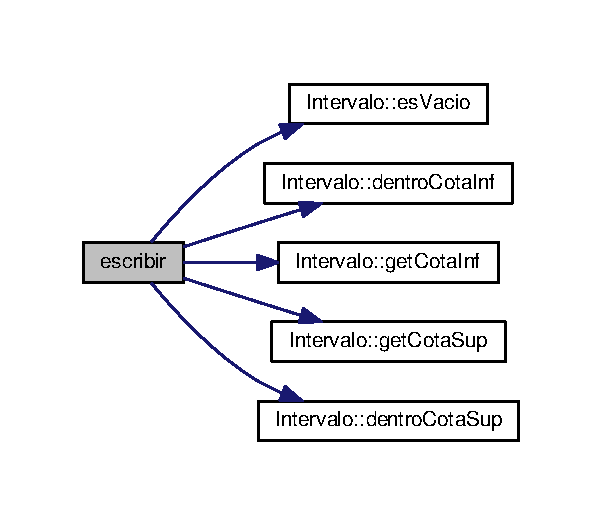
\includegraphics[width=289pt]{intervalo_8h_ae93092259c95b463d176a768b9884802_cgraph}
\end{center}
\end{figure}
\mbox{\Hypertarget{intervalo_8h_ab691781bae666d71c1430e097a742ddb}\label{intervalo_8h_ab691781bae666d71c1430e097a742ddb}} 
\index{intervalo.\+h@{intervalo.\+h}!interseccion@{interseccion}}
\index{interseccion@{interseccion}!intervalo.\+h@{intervalo.\+h}}
\subsubsection{\texorpdfstring{interseccion()}{interseccion()}}
{\footnotesize\ttfamily \hyperlink{classIntervalo}{Intervalo} interseccion (\begin{DoxyParamCaption}\item[{\hyperlink{classIntervalo}{Intervalo}}]{i1,  }\item[{\hyperlink{classIntervalo}{Intervalo}}]{i2 }\end{DoxyParamCaption})}



realiza la interseccion de dos intervalos, puede resultar un intervalo vacío en caso de que no tengan cotas comunes, en caso contrario se revisan las cotas. 


\begin{DoxyParams}{Parámetros}
{\em i1} & primer intervalo de entrada \\
\hline
{\em i2} & segundo intervalo de entrada \\
\hline
\end{DoxyParams}
\begin{DoxyReturn}{Devuelve}
devuelve el intervalo resultante de realizar la interseccion entre los dos intervalos de entrada 
\end{DoxyReturn}
\mbox{\Hypertarget{intervalo_8h_a81ca561257a3eea794e139a64fdd6593}\label{intervalo_8h_a81ca561257a3eea794e139a64fdd6593}} 
\index{intervalo.\+h@{intervalo.\+h}!leer@{leer}}
\index{leer@{leer}!intervalo.\+h@{intervalo.\+h}}
\subsubsection{\texorpdfstring{leer()}{leer()}}
{\footnotesize\ttfamily void leer (\begin{DoxyParamCaption}\item[{\hyperlink{classIntervalo}{Intervalo} \&}]{i }\end{DoxyParamCaption})}



Lee los valores del intervalo según el formato indicado en el guión. 


\begin{DoxyParams}{Parámetros}
{\em i} & El intervalo \\
\hline
\end{DoxyParams}


Definición en la línea 91 del archivo intervalo.\+cpp.


\begin{DoxyCode}
91                           \{
92     \textcolor{comment}{// Formato de lectura del intervalo: [|( x,y )|]}
93     \textcolor{keywordtype}{bool} cerradoInf = \textcolor{keyword}{true};
94     \textcolor{keywordtype}{bool} cerradoSup = \textcolor{keyword}{true};
95     \textcolor{keywordtype}{double} cotaInf, cotaSup;
96     \textcolor{keywordtype}{char} car;
97     cin >> car;
98     \textcolor{keywordflow}{if} (car == \textcolor{charliteral}{'('})
99         cerradoInf = \textcolor{keyword}{false};
100     cin >> cotaInf;
101     cin >> car;
102     cin >> cotaSup;
103     cin >> car;
104     \textcolor{keywordflow}{if} (car == \textcolor{charliteral}{')'})
105         cerradoSup = \textcolor{keyword}{false};
106     obj.setIntervalo(cotaInf, cotaSup, cerradoInf, cerradoSup);
107 \}
\end{DoxyCode}
Gráfico de llamadas para esta función\+:
\nopagebreak
\begin{figure}[H]
\begin{center}
\leavevmode
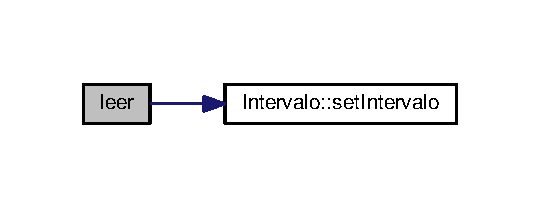
\includegraphics[width=259pt]{intervalo_8h_a81ca561257a3eea794e139a64fdd6593_cgraph}
\end{center}
\end{figure}

\hypertarget{intervalo_8cpp}{}\section{Referencia del Archivo src/intervalo.cpp}
\label{intervalo_8cpp}\index{src/intervalo.\+cpp@{src/intervalo.\+cpp}}
{\ttfamily \#include $<$iostream$>$}\newline
{\ttfamily \#include $<$assert.\+h$>$}\newline
{\ttfamily \#include \char`\"{}intervalo.\+h\char`\"{}}\newline
Dependencia gráfica adjunta para intervalo.\+cpp\+:
\nopagebreak
\begin{figure}[H]
\begin{center}
\leavevmode
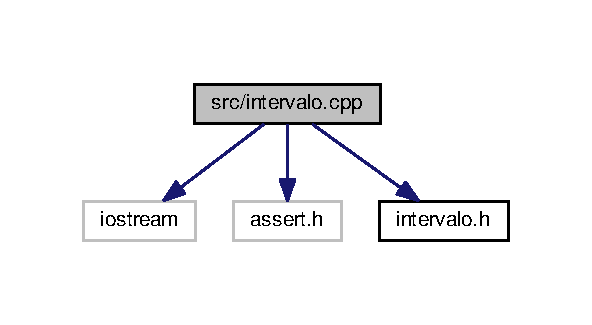
\includegraphics[width=284pt]{intervalo_8cpp__incl}
\end{center}
\end{figure}
\subsection*{Funciones}
\begin{DoxyCompactItemize}
\item 
\mbox{\Hypertarget{intervalo_8cpp_a29f33b0f3e51edc157226a9d47344f5e}\label{intervalo_8cpp_a29f33b0f3e51edc157226a9d47344f5e}} 
bool {\bfseries valido} (double cinf, double csup, bool cerrinf, bool cerrsup)
\item 
void \hyperlink{intervalo_8cpp_a4ffcdcbcf710a7461d8263cd14a32438}{escribir} (const \hyperlink{classIntervalo}{Intervalo} \&obj)
\begin{DoxyCompactList}\small\item\em Imprime los valores de un intervalo de forma visual según lo indicado en el guión. \end{DoxyCompactList}\item 
void \hyperlink{intervalo_8cpp_af4a52a4cb7d127beb07eba78a088f65e}{leer} (\hyperlink{classIntervalo}{Intervalo} \&obj)
\begin{DoxyCompactList}\small\item\em Lee los valores del intervalo según el formato indicado en el guión. \end{DoxyCompactList}\item 
void \hyperlink{intervalo_8cpp_af04754c0b696dbfdab957682cd4af7d2}{comprobar\+Vacio} (\hyperlink{classIntervalo}{Intervalo} obj)
\begin{DoxyCompactList}\small\item\em Muestra un mensaje en pantalla indicando si el intervalo es vacío o no. \end{DoxyCompactList}\end{DoxyCompactItemize}


\subsection{Descripción detallada}
\begin{DoxyAuthor}{Autor}
decsai.\+ugr.\+es 
\end{DoxyAuthor}


\subsection{Documentación de las funciones}
\mbox{\Hypertarget{intervalo_8cpp_af04754c0b696dbfdab957682cd4af7d2}\label{intervalo_8cpp_af04754c0b696dbfdab957682cd4af7d2}} 
\index{intervalo.\+cpp@{intervalo.\+cpp}!comprobar\+Vacio@{comprobar\+Vacio}}
\index{comprobar\+Vacio@{comprobar\+Vacio}!intervalo.\+cpp@{intervalo.\+cpp}}
\subsubsection{\texorpdfstring{comprobar\+Vacio()}{comprobarVacio()}}
{\footnotesize\ttfamily void comprobar\+Vacio (\begin{DoxyParamCaption}\item[{\hyperlink{classIntervalo}{Intervalo}}]{i }\end{DoxyParamCaption})}



Muestra un mensaje en pantalla indicando si el intervalo es vacío o no. 


\begin{DoxyParams}{Parámetros}
{\em i} & El intervalo \\
\hline
\end{DoxyParams}


Definición en la línea 109 del archivo intervalo.\+cpp.


\begin{DoxyCode}
109                                   \{
110      \hyperlink{intervalo_8cpp_a4ffcdcbcf710a7461d8263cd14a32438}{escribir}(obj);
111     \textcolor{keywordflow}{if} (obj.\hyperlink{classIntervalo_adc77e18147f9f9f85476a0d44257bb02}{esVacio}())
112         cout << \textcolor{stringliteral}{"Vacio"};
113     \textcolor{keywordflow}{else}  cout << \textcolor{stringliteral}{"NO Vacio"};
114     cout << endl;
115 \}
\end{DoxyCode}
Gráfico de llamadas para esta función\+:
\nopagebreak
\begin{figure}[H]
\begin{center}
\leavevmode
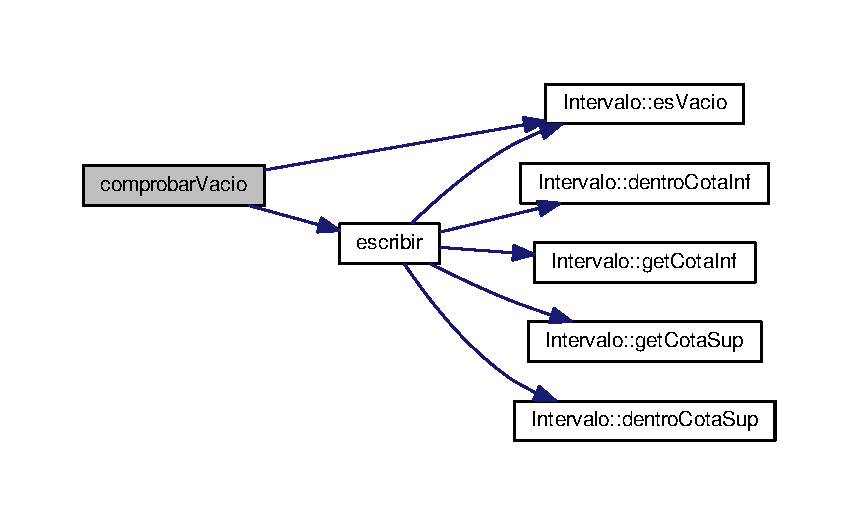
\includegraphics[width=350pt]{intervalo_8cpp_af04754c0b696dbfdab957682cd4af7d2_cgraph}
\end{center}
\end{figure}
\mbox{\Hypertarget{intervalo_8cpp_a4ffcdcbcf710a7461d8263cd14a32438}\label{intervalo_8cpp_a4ffcdcbcf710a7461d8263cd14a32438}} 
\index{intervalo.\+cpp@{intervalo.\+cpp}!escribir@{escribir}}
\index{escribir@{escribir}!intervalo.\+cpp@{intervalo.\+cpp}}
\subsubsection{\texorpdfstring{escribir()}{escribir()}}
{\footnotesize\ttfamily void escribir (\begin{DoxyParamCaption}\item[{const \hyperlink{classIntervalo}{Intervalo} \&}]{i }\end{DoxyParamCaption})}



Imprime los valores de un intervalo de forma visual según lo indicado en el guión. 


\begin{DoxyParams}{Parámetros}
{\em El} & intervalo \\
\hline
\end{DoxyParams}


Definición en la línea 77 del archivo intervalo.\+cpp.


\begin{DoxyCode}
77                                      \{
78     \textcolor{keywordflow}{if} (obj.\hyperlink{classIntervalo_adc77e18147f9f9f85476a0d44257bb02}{esVacio}())
79         cout << \textcolor{stringliteral}{"0 !!"};
80     \textcolor{keywordflow}{else} \{
81         \textcolor{keywordflow}{if} (obj.\hyperlink{classIntervalo_aac8f7b98dd0d702086ea897f5c9ad932}{dentroCotaInf}())
82          cout << \textcolor{charliteral}{'['};
83         \textcolor{keywordflow}{else} cout << \textcolor{charliteral}{'('};
84         cout << obj.\hyperlink{classIntervalo_aafa3f6ec78c6bd44b568e343fb22fc90}{getCotaInf}() << \textcolor{stringliteral}{","} << obj.\hyperlink{classIntervalo_a2dd767a860e4e85ec3d5a44e78884b76}{getCotaSup}();
85         \textcolor{keywordflow}{if} (obj.\hyperlink{classIntervalo_aed0964a68d4b727bd104f5128ee7a7ef}{dentroCotaSup}())
86             cout << \textcolor{charliteral}{']'};
87         \textcolor{keywordflow}{else} cout << \textcolor{charliteral}{')'};
88     \}
89 \}
\end{DoxyCode}
Gráfico de llamadas para esta función\+:
\nopagebreak
\begin{figure}[H]
\begin{center}
\leavevmode
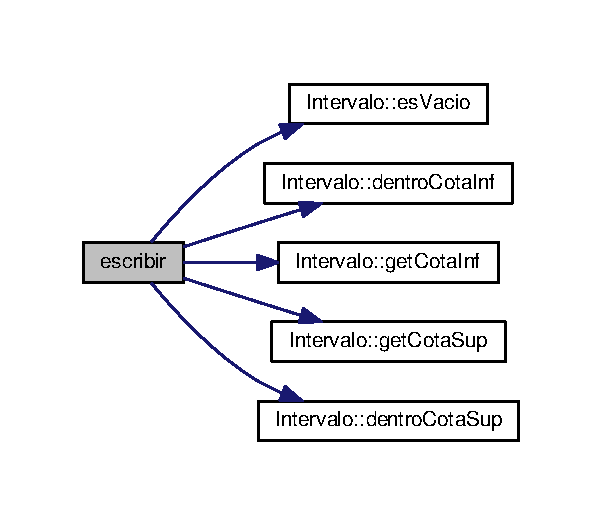
\includegraphics[width=289pt]{intervalo_8cpp_a4ffcdcbcf710a7461d8263cd14a32438_cgraph}
\end{center}
\end{figure}
\mbox{\Hypertarget{intervalo_8cpp_af4a52a4cb7d127beb07eba78a088f65e}\label{intervalo_8cpp_af4a52a4cb7d127beb07eba78a088f65e}} 
\index{intervalo.\+cpp@{intervalo.\+cpp}!leer@{leer}}
\index{leer@{leer}!intervalo.\+cpp@{intervalo.\+cpp}}
\subsubsection{\texorpdfstring{leer()}{leer()}}
{\footnotesize\ttfamily void leer (\begin{DoxyParamCaption}\item[{\hyperlink{classIntervalo}{Intervalo} \&}]{i }\end{DoxyParamCaption})}



Lee los valores del intervalo según el formato indicado en el guión. 


\begin{DoxyParams}{Parámetros}
{\em i} & El intervalo \\
\hline
\end{DoxyParams}


Definición en la línea 91 del archivo intervalo.\+cpp.


\begin{DoxyCode}
91                           \{
92     \textcolor{comment}{// Formato de lectura del intervalo: [|( x,y )|]}
93     \textcolor{keywordtype}{bool} cerradoInf = \textcolor{keyword}{true};
94     \textcolor{keywordtype}{bool} cerradoSup = \textcolor{keyword}{true};
95     \textcolor{keywordtype}{double} cotaInf, cotaSup;
96     \textcolor{keywordtype}{char} car;
97     cin >> car;
98     \textcolor{keywordflow}{if} (car == \textcolor{charliteral}{'('})
99         cerradoInf = \textcolor{keyword}{false};
100     cin >> cotaInf;
101     cin >> car;
102     cin >> cotaSup;
103     cin >> car;
104     \textcolor{keywordflow}{if} (car == \textcolor{charliteral}{')'})
105         cerradoSup = \textcolor{keyword}{false};
106     obj.\hyperlink{classIntervalo_a3e7cfa7c148a4e60be7040fecf506313}{setIntervalo}(cotaInf, cotaSup, cerradoInf, cerradoSup);
107 \}
\end{DoxyCode}
Gráfico de llamadas para esta función\+:
\nopagebreak
\begin{figure}[H]
\begin{center}
\leavevmode
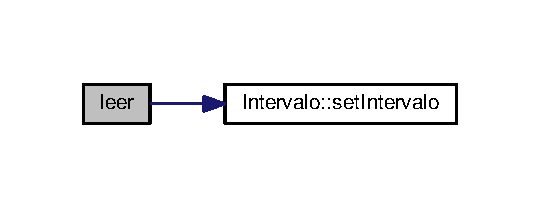
\includegraphics[width=259pt]{intervalo_8cpp_af4a52a4cb7d127beb07eba78a088f65e_cgraph}
\end{center}
\end{figure}

\hypertarget{main_8cpp}{}\section{Referencia del Archivo src/main.cpp}
\label{main_8cpp}\index{src/main.\+cpp@{src/main.\+cpp}}
{\ttfamily \#include $<$iostream$>$}\newline
{\ttfamily \#include \char`\"{}intervalo.\+h\char`\"{}}\newline
Dependencia gráfica adjunta para main.\+cpp\+:
\nopagebreak
\begin{figure}[H]
\begin{center}
\leavevmode
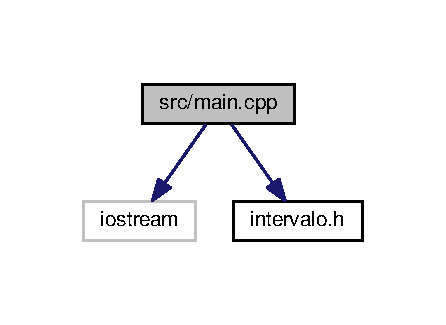
\includegraphics[width=214pt]{main_8cpp__incl}
\end{center}
\end{figure}
\subsection*{Funciones}
\begin{DoxyCompactItemize}
\item 
\mbox{\Hypertarget{main_8cpp_ae66f6b31b5ad750f1fe042a706a4e3d4}\label{main_8cpp_ae66f6b31b5ad750f1fe042a706a4e3d4}} 
int {\bfseries main} ()
\end{DoxyCompactItemize}


\subsection{Descripción detallada}
\begin{DoxyAuthor}{Autor}
decsai.\+ugr.\+es 
\end{DoxyAuthor}

%--- End generated contents ---

% Index
\backmatter
\newpage
\phantomsection
\clearemptydoublepage
\addcontentsline{toc}{chapter}{Índice}
\printindex

\end{document}
